% vim: set textwidth=78 autoindent:
% !TeX root = user_guide.tex

\chapter{Kern-Plugins verwenden}
\label{sec:core_plugins}
\index{Plugins!Kern-Plugins}

% when the revision of a Kapitel has been finalized, 
% comment out the following line:
% \updatedisclaimer


{\setlength{\extrarowheight}{15pt}
\small
\begin{longtable}{|p{1.2cm}|p{3.8cm}|p{7.5cm}|p{3cm}|}
\caption{26 QGIS Kern-Plugins}\label{tab:core_plugins} \\
\hline
 \textbf{Icon} & \textbf{Plugin} & \textbf{Beschreibung} & \textbf{Handbuch Referenz}\\
\endfirsthead
\hline
\textbf{Icon} & \textbf{Plugin} & \textbf{Beschreibung} & \textbf{Handbuch Referenz}\\
\endhead
\hline

\includegraphics[width=0.6cm]{delimited_text}
 & Textdatei als Layer importieren \index{plugins!delimited text} 
 & L�dt und stellt Textdateien in CSV-Format dar, die X- und Y-Koordinaten haben &  Kapitel \ref{label_dltext} \\ 
\hline

\includegraphics[width=0.6cm]{coordinate_capture}
 & Koordinaten aufnehmen \index{plugins!coordinate capture}& Koordinaten in anderem KBS verfolgen & Kapitel \ref{coordcapt} \\
\hline 

\includegraphics[width=0.6cm]{copyright_label}
 & Copyright Label \index{plugins!copyright}& Zeichnet Urheberrechtsinformationen & Kapitel \ref{copyrightlabel} \\
\hline

\includegraphics[width=0.6cm]{plugin}
 & Diagramm �berlagerung \index{plugins!diagram}& Erweiterung, um Diagramme auf Vektorlayer zu setzen & Kapitel \ref{sec:diagram}\\
\hline

\includegraphics[width=0.6cm]{plugin}
 & Verschiebungserweiterung \index{plugins!point displacement}& Erg�nzt neue Darstellung, die Punkte automatisch verschiebt, wenn sie die gleiche Position haben & Kapitel 
\ref{new_generation_sym}\\
\hline
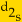
\includegraphics[width=0.6cm]{dxf2shp_converter}
 & DXF2Shape Konverter \index{plugins!DXF2Shape}& Wandelt vom DXF- ins Shapeformat um & Kapitel \ref{dxf2shape}\\
\hline

\includegraphics[width=0.6cm]{plugin}
 & eVis & Ein Ereignisvisualisierungswerkzeug - Bilder anzeigen, die Vektorobjekten zugeordnet sind & Kapitel \ref{sec:evis}\\
\hline

\includegraphics[width=0.6cm, height=0.6cm]{ftoolslogo}
 & fTools \index{plugins!ftools}& Werkzeuge f�r Vektoranalyse und Management & Kapitel \ref{sec:ftools}\\
\hline

\includegraphics[width=0.6cm]{gps_importer}
 & GPS Werkzeuge \index{plugins!gps}& Werkzeuge zum Laden und Importieren von GPS-Daten & Kapitel \ref{label_plugingps}\\
\hline

\includegraphics[width=0.6cm]{grass}
 & GRASS \index{plugin!grass toolbox} & Einbinden von GRASS Daten und Modulen & Kapitel \ref{sec:grass}\\
\hline

\includegraphics[width=0.6cm, height=0.6cm]{raster-info}
 & GDALTools \index{plugins!gdaltools} & Integration von GDAL Tools in QGIS & Kapitel 
\ref{label_plugingdaltools}\\
\hline

\includegraphics[width=0.6cm]{georeferencer}
 & GDAL Georeferenzierung \index{plugin!georeferencer} & Rasterkarten mif GDAL georeferenzieren & Kapitel \ref{sec:georef}\\
\hline

\includegraphics[width=0.6cm]{interpolation}
& Interpolationserweiterung \index{plugins!Interpolation}& St�tzpunktinterpolation von Vektorlayern & Kapitel \ref{sec:interpol}\\
\hline

\includegraphics[width=0.6cm]{mapserver_export}
& MapServer Export \index{plugins!MapServer Export}& Exportieren einer QGIS Projektdatei in einem Mapfile & Kapitel \ref{sec:mapserver_export} \\
\hline

\includegraphics[width=0.6cm]{north_arrow}
& Nordpfeil \index{plugins!north arrow}& Stelle einen Nordpfeil auf der Karte dar & Kapitel \ref{northarrow}\\
\hline

\includegraphics[width=0.6cm]{offline_editing_copy}
 & Offline Editing & Offline-Bearbeitung und Datensynchronisation & Kapitel \ref{sec:offlinedit}\\
\hline
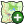
\includegraphics[width=0.6cm]{osm_load}
 & OpenStreetMap & Darstellen und Editieren von OpenStreetMap Daten & Kapitel \ref{plugins_osm}\\
\hline

\includegraphics[width=0.6cm]{oracle_raster}
 & Oracle-Spatial-Georaster \index{plugins!georaster}& Auf OracleSpatial-GeoRaster zugreifen & Kapitel \ref{sec:oracleraster}\\
\hline
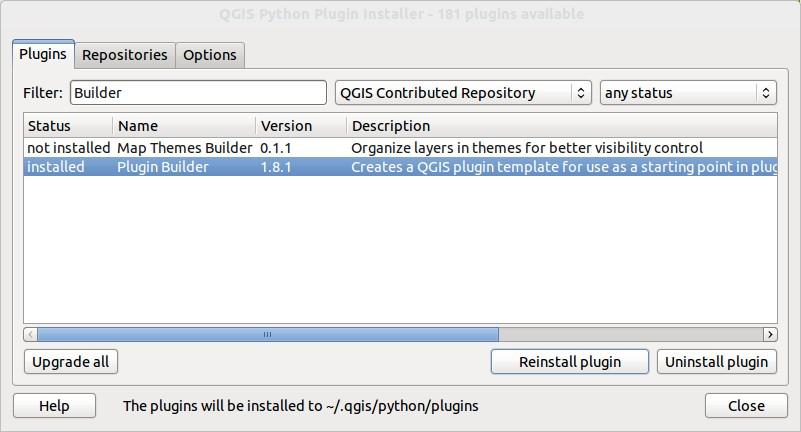
\includegraphics[width=0.6cm]{plugin_installer}
 & Plugin Installer \index{plugins!Plugin Installer} & Herunterladen und Installieren von Python Erweiterungen & Kapitel \ref{sec:python_plugin_installer}\\
\hline

\includegraphics[width=0.6cm]{raster_terrain}
& Rastergel�ndeanalyse \index{plugins!Raster Terrain Modelling}& Erweiterung zur rasterbasierten Gel�ndeanalyse & Kapitel \ref{sec:rasterrain}\\
\hline

\includegraphics[width=0.6cm]{plugin}
 & Stra�engraph Erweiterung \index{plugins!road graph} & L�sen des K�rzeste Wege Problems & Kapitel \ref{sec:roadgraph} \\
\hline

\includegraphics[width=0.6cm]{spiticon}
 & SPIT \index{plugins!spit} & Importieren von Shapefiles nach Postgres/PostGIS & Kapitel \ref{sec:loading_postgis_data} \\
 \hline

\includegraphics[width=0.6cm]{plugin}
 & SQL-Anywhere \index{plugins!SQL anywhere} &  Speichert Vektorlayer in einer SQL-Anywhere Datenbank & Kapitel \ref{sec:sqlanywhere} \\
 \hline

\includegraphics[width=0.6cm]{scale_bar}
 & Ma�stab \index{plugins!scalebar}& Zeichnet einen Ma�stab & Kapitel \ref{scalebar} \\
\hline

\includegraphics[width=0.6cm]{spatialquery}
 & R�umliche Abfrage & R�umliche Abfrage von Vektorlayern & Kapitel \ref{sec:spatial_query} \\
\hline

\includegraphics[width=0.6cm]{mIconAddWfsLayer}
 & WFS-Erweiterung & F�gt einen WFS-LAyer zur Kartendarstellung hinzu & Kapitel \ref{sec:ogc-wfs} \\
\hline
\end{longtable}}



